\documentclass{article}
\usepackage{tikz}
\usepackage{subcaption}
\usepackage{geometry}
\usepackage{xcolor}
\geometry{a4paper, margin=1in}
\begin{document}
\section*{N-Queens Visualization}
\begin{figure}[h!]
\centering
\begin{subfigure}{0.45\textwidth}
\centering
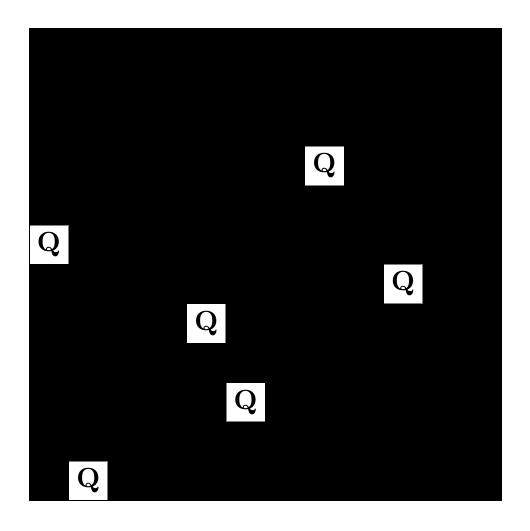
\begin{tikzpicture}[scale=0.5]
\draw[step=1.0,gray,thin] (0,0) grid (12,12);
\fill[black] (0,11) rectangle ++(1,1);
\fill[black] (1,11) rectangle ++(1,1);
\fill[black] (2,11) rectangle ++(1,1);
\fill[black] (3,11) rectangle ++(1,1);
\fill[black] (4,11) rectangle ++(1,1);
\fill[black] (5,11) rectangle ++(1,1);
\fill[black] (6,11) rectangle ++(1,1);
\fill[black] (7,11) rectangle ++(1,1);
\fill[black] (8,11) rectangle ++(1,1);
\fill[black] (9,11) rectangle ++(1,1);
\fill[black] (10,11) rectangle ++(1,1);
\fill[black] (11,11) rectangle ++(1,1);
\fill[black] (0,10) rectangle ++(1,1);
\fill[black] (1,10) rectangle ++(1,1);
\fill[black] (2,10) rectangle ++(1,1);
\fill[black] (3,10) rectangle ++(1,1);
\fill[black] (4,10) rectangle ++(1,1);
\fill[black] (5,10) rectangle ++(1,1);
\fill[black] (6,10) rectangle ++(1,1);
\fill[black] (7,10) rectangle ++(1,1);
\fill[black] (8,10) rectangle ++(1,1);
\fill[black] (9,10) rectangle ++(1,1);
\fill[black] (10,10) rectangle ++(1,1);
\fill[black] (11,10) rectangle ++(1,1);
\fill[black] (0,9) rectangle ++(1,1);
\fill[black] (1,9) rectangle ++(1,1);
\fill[black] (2,9) rectangle ++(1,1);
\fill[black] (3,9) rectangle ++(1,1);
\fill[black] (4,9) rectangle ++(1,1);
\fill[black] (5,9) rectangle ++(1,1);
\fill[black] (6,9) rectangle ++(1,1);
\fill[black] (7,9) rectangle ++(1,1);
\fill[black] (8,9) rectangle ++(1,1);
\fill[black] (9,9) rectangle ++(1,1);
\fill[black] (10,9) rectangle ++(1,1);
\fill[black] (11,9) rectangle ++(1,1);
\fill[black] (0,8) rectangle ++(1,1);
\fill[black] (1,8) rectangle ++(1,1);
\fill[black] (2,8) rectangle ++(1,1);
\fill[black] (3,8) rectangle ++(1,1);
\fill[black] (4,8) rectangle ++(1,1);
\fill[black] (5,8) rectangle ++(1,1);
\fill[black] (6,8) rectangle ++(1,1);
\node at (7+0.5, 8+0.5) {\textbf{Q}};
\fill[black] (8,8) rectangle ++(1,1);
\fill[black] (9,8) rectangle ++(1,1);
\fill[black] (10,8) rectangle ++(1,1);
\fill[black] (11,8) rectangle ++(1,1);
\fill[black] (0,7) rectangle ++(1,1);
\fill[black] (1,7) rectangle ++(1,1);
\fill[black] (2,7) rectangle ++(1,1);
\fill[black] (3,7) rectangle ++(1,1);
\fill[black] (4,7) rectangle ++(1,1);
\fill[black] (5,7) rectangle ++(1,1);
\fill[black] (6,7) rectangle ++(1,1);
\fill[black] (7,7) rectangle ++(1,1);
\fill[black] (8,7) rectangle ++(1,1);
\fill[black] (9,7) rectangle ++(1,1);
\fill[black] (10,7) rectangle ++(1,1);
\fill[black] (11,7) rectangle ++(1,1);
\node at (0+0.5, 6+0.5) {\textbf{Q}};
\fill[black] (1,6) rectangle ++(1,1);
\fill[black] (2,6) rectangle ++(1,1);
\fill[black] (3,6) rectangle ++(1,1);
\fill[black] (4,6) rectangle ++(1,1);
\fill[black] (5,6) rectangle ++(1,1);
\fill[black] (6,6) rectangle ++(1,1);
\fill[black] (7,6) rectangle ++(1,1);
\fill[black] (8,6) rectangle ++(1,1);
\fill[black] (9,6) rectangle ++(1,1);
\fill[black] (10,6) rectangle ++(1,1);
\fill[black] (11,6) rectangle ++(1,1);
\fill[black] (0,5) rectangle ++(1,1);
\fill[black] (1,5) rectangle ++(1,1);
\fill[black] (2,5) rectangle ++(1,1);
\fill[black] (3,5) rectangle ++(1,1);
\fill[black] (4,5) rectangle ++(1,1);
\fill[black] (5,5) rectangle ++(1,1);
\fill[black] (6,5) rectangle ++(1,1);
\fill[black] (7,5) rectangle ++(1,1);
\fill[black] (8,5) rectangle ++(1,1);
\node at (9+0.5, 5+0.5) {\textbf{Q}};
\fill[black] (10,5) rectangle ++(1,1);
\fill[black] (11,5) rectangle ++(1,1);
\fill[black] (0,4) rectangle ++(1,1);
\fill[black] (1,4) rectangle ++(1,1);
\fill[black] (2,4) rectangle ++(1,1);
\fill[black] (3,4) rectangle ++(1,1);
\node at (4+0.5, 4+0.5) {\textbf{Q}};
\fill[black] (5,4) rectangle ++(1,1);
\fill[black] (6,4) rectangle ++(1,1);
\fill[black] (7,4) rectangle ++(1,1);
\fill[black] (8,4) rectangle ++(1,1);
\fill[black] (9,4) rectangle ++(1,1);
\fill[black] (10,4) rectangle ++(1,1);
\fill[black] (11,4) rectangle ++(1,1);
\fill[black] (0,3) rectangle ++(1,1);
\fill[black] (1,3) rectangle ++(1,1);
\fill[black] (2,3) rectangle ++(1,1);
\fill[black] (3,3) rectangle ++(1,1);
\fill[black] (4,3) rectangle ++(1,1);
\fill[black] (5,3) rectangle ++(1,1);
\fill[black] (6,3) rectangle ++(1,1);
\fill[black] (7,3) rectangle ++(1,1);
\fill[black] (8,3) rectangle ++(1,1);
\fill[black] (9,3) rectangle ++(1,1);
\fill[black] (10,3) rectangle ++(1,1);
\fill[black] (11,3) rectangle ++(1,1);
\fill[black] (0,2) rectangle ++(1,1);
\fill[black] (1,2) rectangle ++(1,1);
\fill[black] (2,2) rectangle ++(1,1);
\fill[black] (3,2) rectangle ++(1,1);
\fill[black] (4,2) rectangle ++(1,1);
\node at (5+0.5, 2+0.5) {\textbf{Q}};
\fill[black] (6,2) rectangle ++(1,1);
\fill[black] (7,2) rectangle ++(1,1);
\fill[black] (8,2) rectangle ++(1,1);
\fill[black] (9,2) rectangle ++(1,1);
\fill[black] (10,2) rectangle ++(1,1);
\fill[black] (11,2) rectangle ++(1,1);
\fill[black] (0,1) rectangle ++(1,1);
\fill[black] (1,1) rectangle ++(1,1);
\fill[black] (2,1) rectangle ++(1,1);
\fill[black] (3,1) rectangle ++(1,1);
\fill[black] (4,1) rectangle ++(1,1);
\fill[black] (5,1) rectangle ++(1,1);
\fill[black] (6,1) rectangle ++(1,1);
\fill[black] (7,1) rectangle ++(1,1);
\fill[black] (8,1) rectangle ++(1,1);
\fill[black] (9,1) rectangle ++(1,1);
\fill[black] (10,1) rectangle ++(1,1);
\fill[black] (11,1) rectangle ++(1,1);
\fill[black] (0,0) rectangle ++(1,1);
\node at (1+0.5, 0+0.5) {\textbf{Q}};
\fill[black] (2,0) rectangle ++(1,1);
\fill[black] (3,0) rectangle ++(1,1);
\fill[black] (4,0) rectangle ++(1,1);
\fill[black] (5,0) rectangle ++(1,1);
\fill[black] (6,0) rectangle ++(1,1);
\fill[black] (7,0) rectangle ++(1,1);
\fill[black] (8,0) rectangle ++(1,1);
\fill[black] (9,0) rectangle ++(1,1);
\fill[black] (10,0) rectangle ++(1,1);
\fill[black] (11,0) rectangle ++(1,1);
\draw (0,0) rectangle (12,12);
\end{tikzpicture}
\caption{Input (50.0\% Queens Masked)}
\end{subfigure}
\hfill
\begin{subfigure}{0.45\textwidth}
\centering
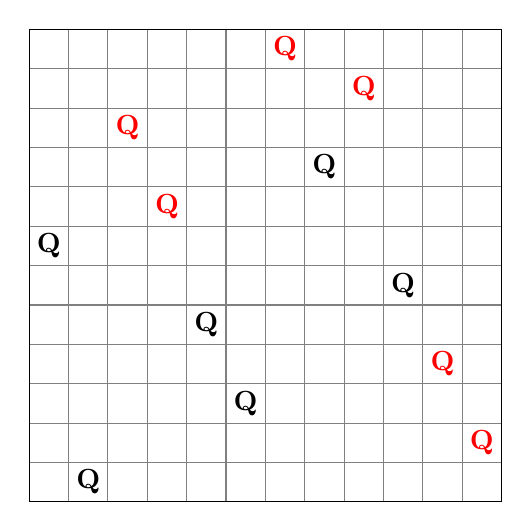
\begin{tikzpicture}[scale=0.5]
\draw[step=1.0,gray,thin] (0,0) grid (12,12);
\node[red] at (6+0.5, 11+0.5) {\textbf{Q}};
\node[red] at (8+0.5, 10+0.5) {\textbf{Q}};
\node[red] at (2+0.5, 9+0.5) {\textbf{Q}};
\node at (7+0.5, 8+0.5) {\textbf{Q}};
\node[red] at (3+0.5, 7+0.5) {\textbf{Q}};
\node at (0+0.5, 6+0.5) {\textbf{Q}};
\node at (9+0.5, 5+0.5) {\textbf{Q}};
\node at (4+0.5, 4+0.5) {\textbf{Q}};
\node[red] at (10+0.5, 3+0.5) {\textbf{Q}};
\node at (5+0.5, 2+0.5) {\textbf{Q}};
\node[red] at (11+0.5, 1+0.5) {\textbf{Q}};
\node at (1+0.5, 0+0.5) {\textbf{Q}};
\draw (0,0) rectangle (12,12);
\end{tikzpicture}
\caption{Target (Red = Inferred)}
\end{subfigure}
\end{figure}
\end{document}